\SourceLeaf{278}
\begin{center}
{\Large\bfseries\textls{NACHLASS.}}\par\medskip
[I.]

\bigskip \textbf{[ZUR GEOMETRIA SITUS.]}

\bigskip [1.]

\medskip \textbf{THEOREM AUS DER GEOMETRIA SITUS.}
\end{center}

Es sei die Amplitudo einer ganzen in sich selbst zurückkehrenden Curve
$=\pm n\,.\,360^0$. Sie hat wenigstens Knoten
\[
\begin{array}{r@{\quad}rrrrrrrr}
&1&0&1&2&3&4&5&6\\
\text{für }n={}&0&1&2&3&4&5&6&7.
\end{array}
\]
Der Beweis scheint nicht leicht zu sein; wahrscheinlich wird dazu dienen, dass man die Curve ihrem Laufe nach in Theile abtheilt, deren Grenzen die Punkte sind, in denen ihre Richtung $=90^0(2n+1)$, dann eine unendliche gerade Linie, deren Richtung $=90^0$, in der Richtung $0^0$ durch die Fläche schiebt und die Folge der Stücke gehörig beachtet. So ist für diese Curve das Schema folgendes:

\begin{center}
\begin{minipage}{8cm}\centering
\resizebox{8.0cm}{!}{%
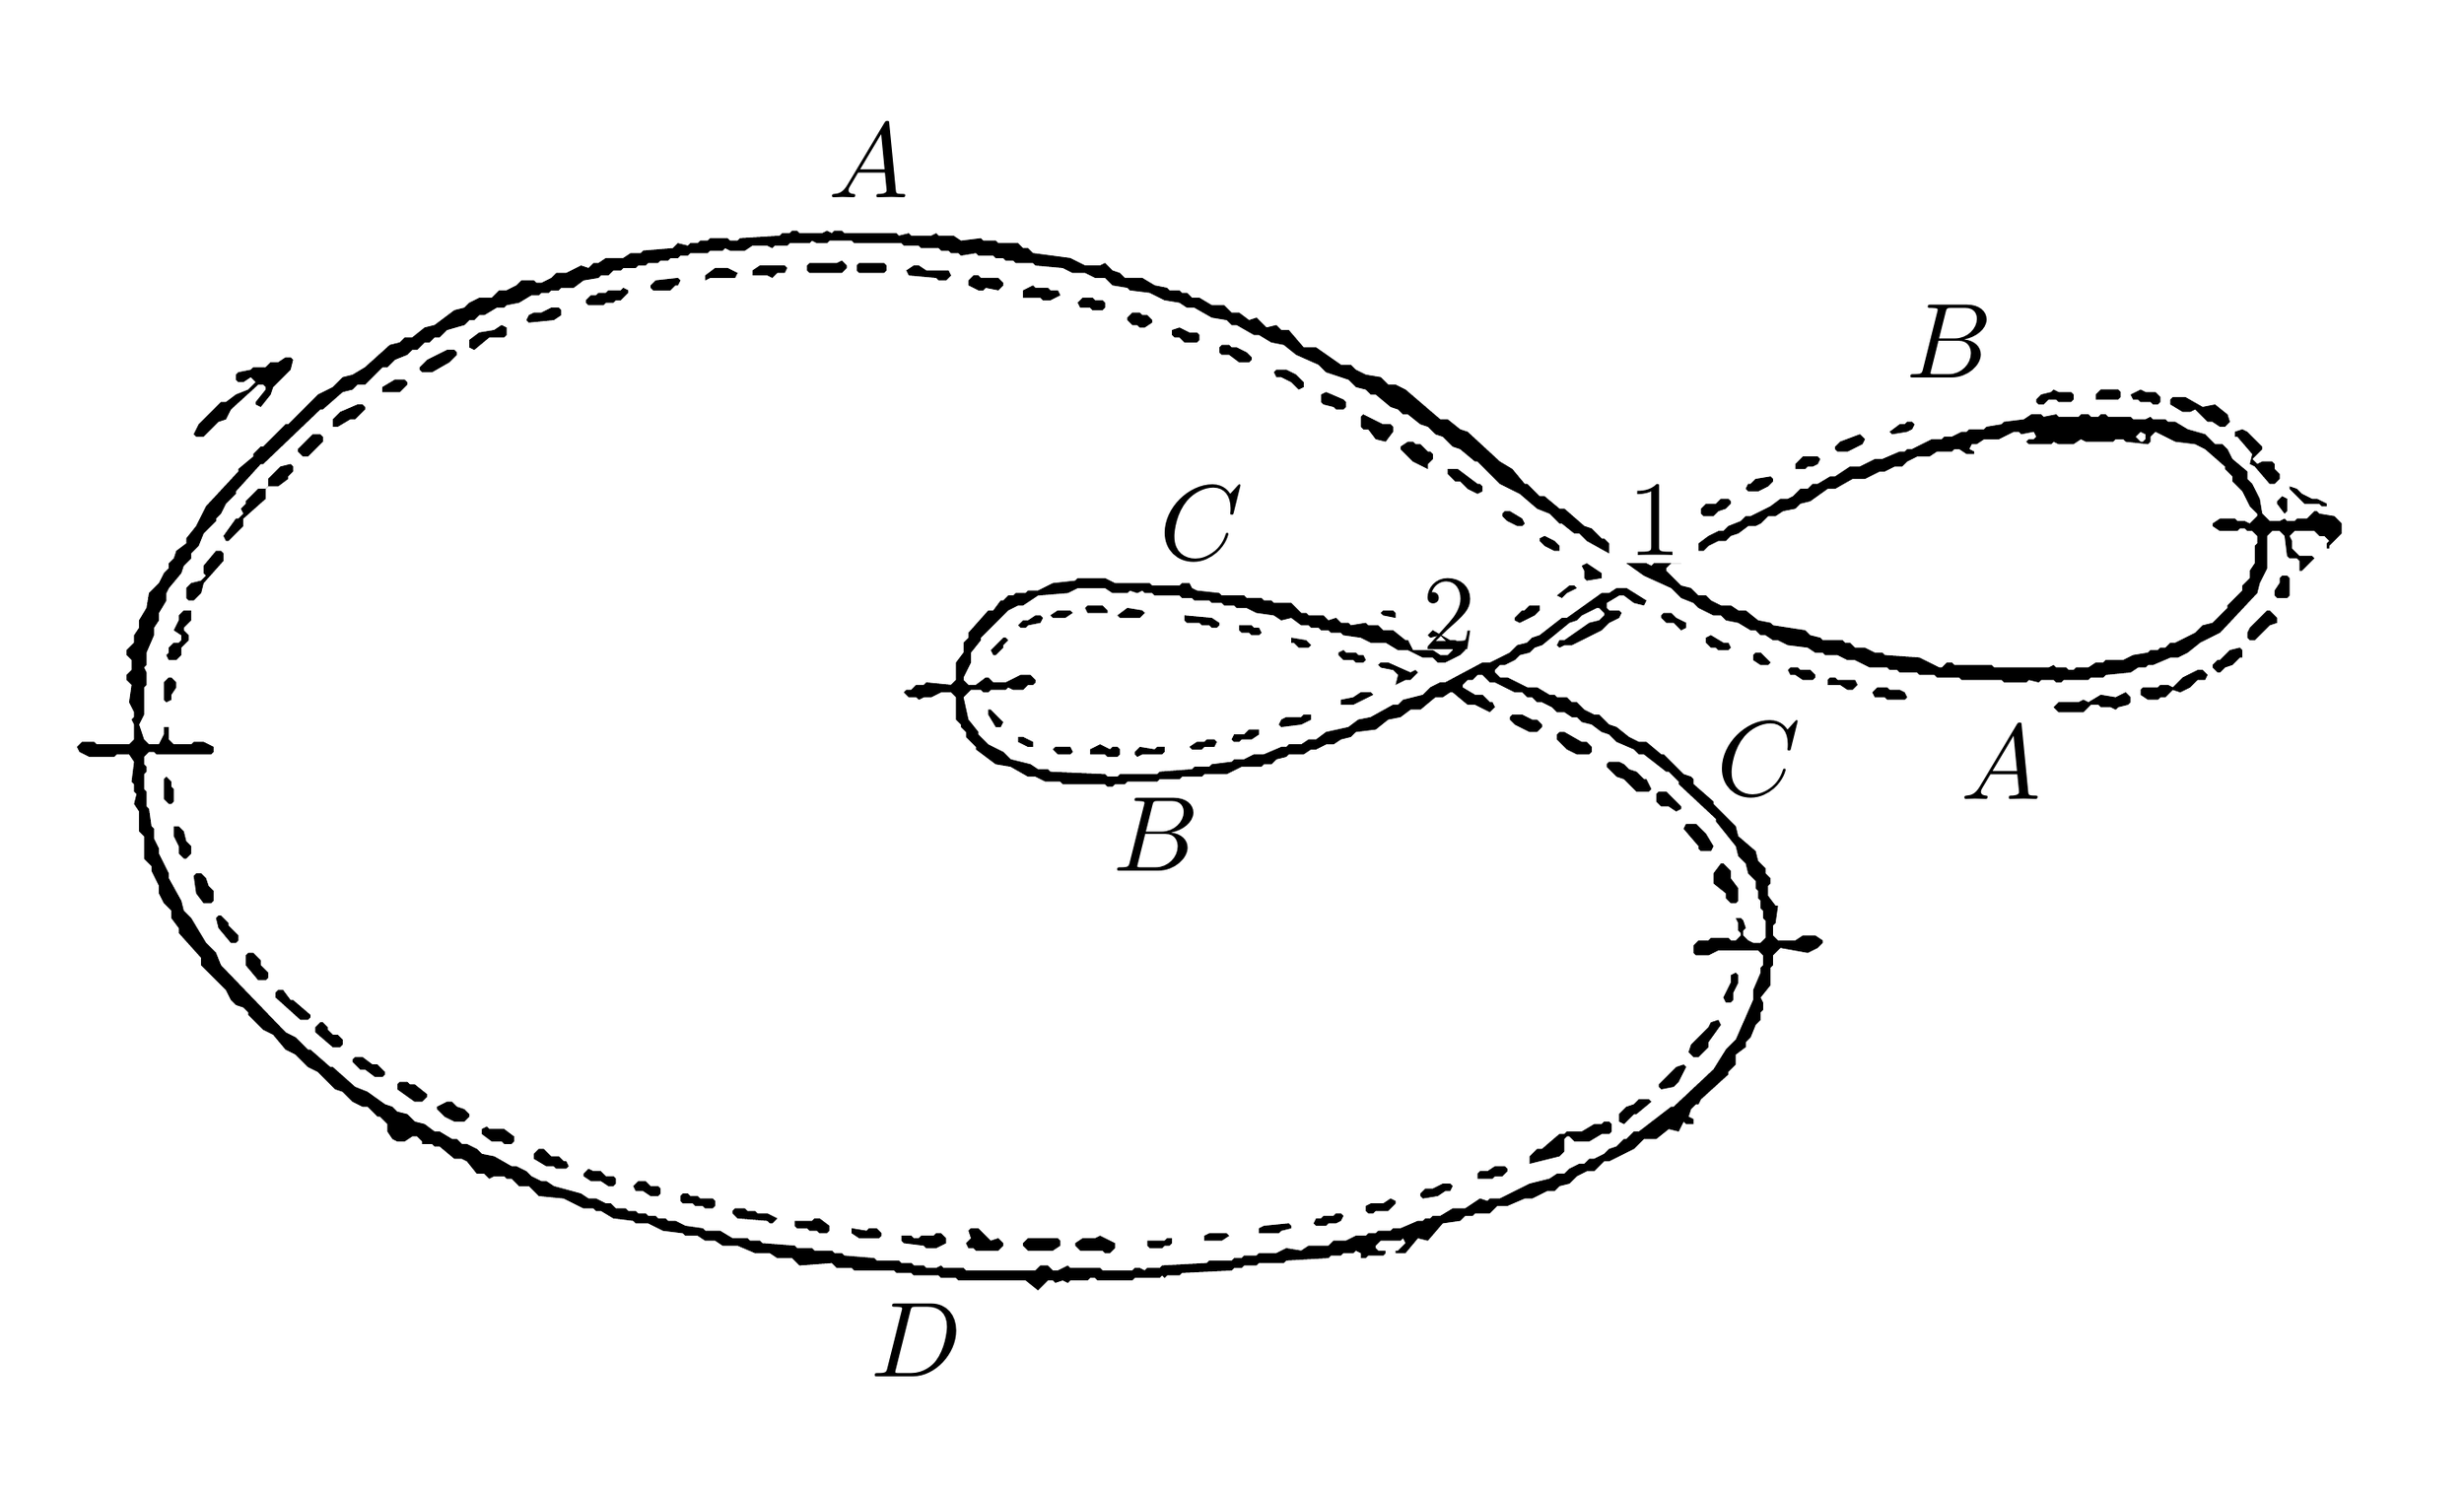
\begin{tikzpicture}[x=1pt,y=-1pt]
\path[use as bounding box] (0,0) rectangle (972,581);
\path[fill=black,draw=none,even odd rule]
(462,489) -- (460,489) -- (459,490) -- (452,490) -- (452,492) -- (453,493) -- (458,493) -- (459,492) -- (461,492) -- (462,491) -- cycle
(402,491) -- (402,492) -- (404,494) -- (414,494) -- (417,492) -- (417,490) -- (416,489) -- (404,489) -- cycle
(439,493) -- (439,491) -- (433,488) -- (431,489) -- (426,489) -- (423,491) -- (423,492) -- (425,494) -- (434,494) -- (435,495) -- (437,495) -- cycle
(475,490) -- (482,490) -- (485,488) -- (484,487) -- (477,487) -- (475,488) -- cycle
(371,491) -- (371,489) -- (369,487) -- (367,487) -- (366,488) -- (361,488) -- (360,489) -- (358,489) -- (357,488) -- (353,488) -- (353,490) -- (354,491) -- (362,492) -- (363,493) -- (367,493) -- cycle
(380,486) -- (381,489) -- (379,491) -- (380,493) -- (382,493) -- (383,494) -- (392,494) -- (394,492) -- (394,491) -- (392,489) -- (389,490) -- (384,485) -- (381,485) -- cycle
(333,485) -- (333,487) -- (336,489) -- (344,489) -- (345,488) -- (345,487) -- (343,485) -- (340,485) -- (339,486) -- cycle
(510,484) -- (509,483) -- (499,484) -- (497,485) -- (497,487) -- (505,487) -- (506,486) -- (510,485) -- cycle
(324,486) -- (324,484) -- (320,481) -- (318,481) -- (317,482) -- (310,482) -- (310,484) -- (311,485) -- (315,485) -- (316,486) -- (319,486) -- (320,487) -- (323,487) -- cycle
(531,480) -- (530,479) -- (528,479) -- (527,480) -- (523,480) -- (522,481) -- (520,481) -- (519,483) -- (520,484) -- (524,484) -- (525,483) -- (528,483) -- (530,482) -- cycle
(285,478) -- (285,479) -- (287,481) -- (299,482) -- (300,483) -- (301,483) -- (303,481) -- (299,479) -- (295,479) -- (294,478) -- (291,478) -- (290,477) -- (286,477) -- cycle
(552,474) -- (550,473) -- (547,475) -- (542,475) -- (540,476) -- (540,478) -- (541,479) -- (543,479) -- (544,478) -- (549,478) -- (552,475) -- cycle
(264,472) -- (264,474) -- (265,475) -- (269,475) -- (270,476) -- (273,476) -- (274,477) -- (277,477) -- (278,476) -- (278,474) -- (277,473) -- (272,473) -- (271,472) -- (268,472) -- (267,471) -- (265,471) -- cycle
(575,468) -- (574,467) -- (571,467) -- (567,469) -- (564,469) -- (562,471) -- (562,472) -- (563,473) -- (569,472) -- (572,470) -- (574,470) -- cycle
(245,468) -- (246,470) -- (249,470) -- (252,472) -- (255,472) -- (256,471) -- (256,469) -- (255,468) -- (252,468) -- (250,466) -- (247,466) -- cycle
(225,463) -- (225,464) -- (228,466) -- (232,466) -- (235,468) -- (237,468) -- (238,467) -- (238,465) -- (237,464) -- (234,464) -- (232,462) -- (229,462) -- (227,461) -- cycle
(597,461) -- (596,460) -- (592,460) -- (589,462) -- (586,462) -- (585,463) -- (585,465) -- (591,465) -- (592,464) -- (595,464) -- (597,462) -- cycle
(205,455) -- (205,457) -- (210,460) -- (213,460) -- (214,461) -- (218,461) -- (219,460) -- (218,458) -- (217,458) -- (215,456) -- (212,456) -- (209,453) -- (207,453) -- cycle
(184,445) -- (184,447) -- (188,450) -- (192,450) -- (193,451) -- (196,451) -- (197,450) -- (197,448) -- (193,445) -- (187,445) -- (186,444) -- cycle
(639,443) -- (638,442) -- (636,442) -- (635,443) -- (632,443) -- (627,446) -- (621,446) -- (620,447) -- (618,447) -- (611,453) -- (609,453) -- (606,456) -- (606,459) -- (618,456) -- (620,454) -- (620,449) -- (621,448) -- (622,448) -- (624,450) -- (630,450) -- (635,447) -- (638,447) -- (639,446) -- cycle
(166,436) -- (166,437) -- (169,440) -- (173,442) -- (177,442) -- (179,440) -- (179,439) -- (177,437) -- (174,436) -- (172,434) -- (170,434) -- cycle
(655,434) -- (654,433) -- (650,433) -- (648,435) -- (645,436) -- (642,439) -- (642,442) -- (644,443) -- (648,439) -- (649,439) -- cycle
(150,427) -- (150,429) -- (157,434) -- (160,434) -- (162,432) -- (162,431) -- (157,427) -- (155,427) -- (154,426) -- (151,426) -- cycle
(669,420) -- (668,419) -- (665,420) -- (658,427) -- (658,428) -- (659,429) -- (664,428) -- (666,426) -- cycle
(132,417) -- (132,418) -- (135,421) -- (137,421) -- (141,424) -- (144,424) -- (145,423) -- (145,422) -- (142,419) -- (140,419) -- (136,416) -- (133,416) -- cycle
(119,402) -- (117,404) -- (117,406) -- (124,412) -- (127,412) -- (128,411) -- (128,409) -- (126,407) -- (124,407) -- (122,405) -- (122,404) -- (120,402) -- cycle
(682,401) -- (679,402) -- (678,404) -- (671,411) -- (670,414) -- (672,416) -- (674,416) -- (678,412) -- (678,410) -- (683,403) -- cycle
(101,390) -- (101,392) -- (111,401) -- (114,401) -- (115,400) -- (115,399) -- (108,393) -- (107,393) -- (104,389) -- (102,389) -- cycle
(689,382) -- (687,383) -- (687,386) -- (684,392) -- (685,394) -- (687,394) -- (688,393) -- (688,390) -- (690,386) -- (690,383) -- cycle
(90,374) -- (89,375) -- (89,379) -- (94,385) -- (97,385) -- (98,384) -- (98,382) -- (95,379) -- (95,377) -- (92,374) -- cycle
(78,359) -- (77,360) -- (78,364) -- (83,370) -- (85,370) -- (86,369) -- (86,367) -- (82,363) -- (82,362) -- (79,359) -- cycle
(69,342) -- (68,343) -- (69,350) -- (72,354) -- (75,354) -- (76,353) -- (76,349) -- (74,347) -- (73,344) -- (71,342) -- cycle
(683,338) -- (680,342) -- (680,346) -- (685,350) -- (685,352) -- (687,354) -- (689,354) -- (690,353) -- (690,348) -- (687,344) -- (687,341) -- (684,338) -- cycle
(60,323) -- (60,327) -- (62,331) -- (62,334) -- (64,336) -- (65,336) -- (67,334) -- (67,331) -- (65,329) -- (64,325) -- (62,323) -- cycle
(669,322) -- (668,324) -- (674,331) -- (674,332) -- (675,333) -- (679,333) -- (680,331) -- (677,326) -- (673,322) -- cycle
(657,310) -- (657,313) -- (659,315) -- (662,315) -- (665,317) -- (667,316) -- (667,315) -- (661,309) -- (658,309) -- cycle
(57,303) -- (56,304) -- (56,312) -- (58,314) -- (59,314) -- (60,313) -- (60,308) -- (59,307) -- (59,305) -- cycle
(637,298) -- (637,299) -- (641,303) -- (644,304) -- (649,309) -- (654,309) -- (655,308) -- (653,304) -- (652,304) -- (649,301) -- (646,300) -- (644,298) -- (642,297) -- (638,297) -- cycle
(447,294) -- (448,295) -- (450,294) -- (458,294) -- (459,293) -- (459,291) -- (456,291) -- (455,292) -- (449,291) -- (447,293) -- cycle
(414,292) -- (416,294) -- (421,294) -- (422,293) -- (421,291) -- (415,291) -- cycle
(429,292) -- (429,294) -- (435,294) -- (436,295) -- (440,295) -- (441,294) -- (441,292) -- (440,291) -- (438,291) -- (437,292) -- (433,290) -- cycle
(480,289) -- (479,288) -- (476,288) -- (475,289) -- (472,289) -- (469,291) -- (470,292) -- (474,292) -- (475,291) -- (479,291) -- cycle
(400,287) -- (400,289) -- (404,291) -- (406,291) -- (406,289) -- (402,287) -- cycle
(617,286) -- (617,288) -- (621,292) -- (625,294) -- (630,294) -- (631,293) -- (631,291) -- (629,289) -- (627,289) -- (620,285) -- (618,285) -- cycle
(497,284) -- (493,284) -- (491,286) -- (487,286) -- (486,288) -- (487,289) -- (489,289) -- (490,288) -- (494,288) -- (497,286) -- cycle
(598,279) -- (598,280) -- (600,282) -- (606,285) -- (609,285) -- (611,283) -- (611,282) -- (609,280) -- (607,280) -- (603,278) -- (599,278) -- cycle
(518,278) -- (515,278) -- (514,279) -- (508,279) -- (506,280) -- (505,282) -- (506,283) -- (514,282) -- (518,280) -- cycle
(388,276) -- (388,278) -- (391,283) -- (393,283) -- (394,281) -- (389,276) -- cycle
(848,271) -- (846,269) -- (842,271) -- (836,270) -- (831,273) -- (829,272) -- (827,273) -- (819,273) -- (817,275) -- (819,277) -- (829,277) -- (832,274) -- (835,274) -- (836,275) -- (840,275) -- (842,276) -- (843,275) -- (847,274) -- (848,273) -- cycle
(543,270) -- (542,269) -- (538,269) -- (535,271) -- (530,272) -- (530,274) -- (535,274) -- cycle
(744,269) -- (745,271) -- (749,271) -- (750,272) -- (757,272) -- (758,271) -- (757,269) -- (755,268) -- (751,268) -- (750,267) -- (746,267) -- cycle
(726,264) -- (726,266) -- (731,266) -- (734,268) -- (736,268) -- (738,266) -- (737,264) -- (730,264) -- (729,263) -- (727,263) -- cycle
(59,263) -- (58,263) -- (56,265) -- (56,272) -- (57,273) -- (59,272) -- (59,270) -- (61,267) -- (61,265) -- cycle
(879,262) -- (877,260) -- (875,260) -- (869,263) -- (865,267) -- (863,266) -- (860,266) -- (859,267) -- (853,267) -- (852,268) -- (852,270) -- (855,272) -- (859,272) -- (860,271) -- (862,271) -- (865,268) -- (868,269) -- (872,267) -- (875,264) -- (878,264) -- cycle
(710,260) -- (711,262) -- (713,262) -- (716,264) -- (720,264) -- (721,263) -- (721,262) -- (719,260) -- (715,260) -- (714,259) -- (711,259) -- cycle
(545,258) -- (546,259) -- (551,260) -- (553,262) -- (552,266) -- (556,264) -- (558,264) -- (561,261) -- (560,260) -- (558,261) -- (549,257) -- (546,257) -- cycle
(696,254) -- (696,256) -- (699,258) -- (702,258) -- (703,257) -- (699,253) -- (697,253) -- cycle
(529,253) -- (529,254) -- (531,256) -- (535,256) -- (536,257) -- (539,257) -- (540,256) -- (539,254) -- (537,254) -- (536,253) -- (532,253) -- (531,252) -- cycle
(893,252) -- (892,251) -- (888,252) -- (884,256) -- (883,256) -- (881,258) -- (881,259) -- (883,261) -- (884,261) -- (886,259) -- (889,258) -- (892,255) -- (893,255) -- cycle
(510,247) -- (510,249) -- (511,249) -- (513,251) -- (517,251) -- (518,250) -- (516,248) -- cycle
(395,247) -- (394,247) -- (389,252) -- (390,254) -- (391,254) -- (394,251) -- (394,250) -- (396,248) -- cycle
(677,247) -- (677,249) -- (679,251) -- (681,251) -- (682,252) -- (686,252) -- (687,251) -- (686,249) -- (684,249) -- (679,246) -- cycle
(489,242) -- (489,244) -- (490,245) -- (493,245) -- (494,246) -- (497,246) -- (498,245) -- (497,243) -- (495,243) -- (494,242) -- cycle
(467,238) -- (467,240) -- (468,241) -- (473,241) -- (474,242) -- (477,242) -- (478,243) -- (480,243) -- (481,242) -- (481,241) -- (478,239) -- cycle
(410,239) -- (409,238) -- (407,238) -- (404,240) -- (402,240) -- (400,242) -- (401,243) -- (403,243) -- (404,242) -- (409,241) -- cycle
(659,238) -- (659,239) -- (661,241) -- (664,241) -- (667,244) -- (669,243) -- (669,241) -- (665,239) -- (663,237) -- (660,237) -- cycle
(904,236) -- (903,236) -- (896,243) -- (895,245) -- (895,247) -- (896,248) -- (898,248) -- (904,242) -- (907,241) -- (907,239) -- cycle
(546,237) -- (547,238) -- (552,239) -- (552,237) -- (551,236) -- (547,236) -- cycle
(413,238) -- (414,239) -- (419,239) -- (422,237) -- (421,236) -- (416,236) -- cycle
(67,236) -- (64,236) -- (62,238) -- (62,240) -- (60,244) -- (63,246) -- (63,248) -- (62,249) -- (60,249) -- (58,251) -- (58,253) -- (57,254) -- (58,256) -- (61,256) -- (63,254) -- (63,251) -- (66,248) -- (66,246) -- (64,244) -- (64,243) -- (67,240) -- cycle
(440,238) -- (441,239) -- (449,239) -- (451,237) -- (450,236) -- (444,235) -- cycle
(610,234) -- (606,234) -- (604,236) -- (603,236) -- (600,239) -- (600,240) -- (602,241) -- (608,238) -- (610,236) -- cycle
(427,235) -- (428,237) -- (436,237) -- (436,236) -- (434,234) -- (428,234) -- cycle
(625,227) -- (624,226) -- (622,226) -- (617,230) -- (619,231) -- (621,229) -- cycle
(911,222) -- (909,222) -- (908,223) -- (908,225) -- (906,228) -- (906,230) -- (907,231) -- (911,231) -- (912,230) -- (912,223) -- cycle
(627,218) -- (628,220) -- (628,223) -- (629,224) -- (635,223) -- (635,221) -- (629,217) -- cycle
(79,212) -- (77,212) -- (72,218) -- (72,221) -- (73,222) -- (71,224) -- (67,225) -- (65,227) -- (65,231) -- (66,232) -- (68,232) -- (71,229) -- (72,225) -- (80,216) -- (80,213) -- cycle
(610,207) -- (610,208) -- (612,210) -- (616,212) -- (618,212) -- (618,210) -- (616,208) -- (612,206) -- cycle
(595,197) -- (595,198) -- (597,200) -- (601,202) -- (603,202) -- (604,201) -- (603,199) -- (598,196) -- (596,196) -- cycle
(687,192) -- (686,191) -- (683,191) -- (681,193) -- (677,193) -- (675,195) -- (675,197) -- (676,198) -- (680,198) -- (682,196) -- (685,195) -- (687,193) -- cycle
(909,190) -- (907,192) -- (907,193) -- (910,197) -- (911,196) -- (911,191) -- cycle
(912,186) -- (912,187) -- (918,193) -- (924,193) -- (925,194) -- (927,194) -- (927,193) -- (923,191) -- (921,191) -- (917,189) -- (915,187) -- cycle
(704,183) -- (703,182) -- (697,183) -- (695,185) -- (694,185) -- (693,187) -- (694,188) -- (698,188) -- (702,186) -- (704,184) -- cycle
(573,179) -- (573,181) -- (576,184) -- (578,184) -- (581,187) -- (585,189) -- (587,188) -- (587,186) -- (586,185) -- (585,185) -- (577,179) -- cycle
(107,177) -- (103,178) -- (98,183) -- (98,186) -- (97,187) -- (94,187) -- (89,192) -- (89,193) -- (87,195) -- (88,197) -- (86,199) -- (85,199) -- (80,206) -- (81,208) -- (82,208) -- (88,202) -- (88,199) -- (97,191) -- (97,187) -- (98,186) -- (102,186) -- (106,183) -- (106,182) -- (108,180) -- (108,178) -- cycle
(713,179) -- (717,179) -- (718,178) -- (720,178) -- (722,177) -- (723,175) -- (722,174) -- (716,174) -- (713,177) -- cycle
(554,170) -- (554,171) -- (559,176) -- (565,179) -- (565,177) -- (567,175) -- (567,173) -- (566,172) -- (565,172) -- (562,169) -- (560,169) -- (559,168) -- (557,168) -- cycle
(741,167) -- (739,165) -- (731,168) -- (729,170) -- (729,171) -- (730,172) -- (734,172) -- (740,169) -- cycle
(119,165) -- (116,165) -- (110,171) -- (110,172) -- (112,174) -- (114,174) -- (120,168) -- (120,166) -- cycle
(890,164) -- (890,166) -- (891,166) -- (897,173) -- (896,177) -- (898,178) -- (904,185) -- (906,185) -- (908,183) -- (908,181) -- (906,179) -- (906,177) -- (905,176) -- (901,176) -- (899,177) -- (897,175) -- (901,171) -- (901,170) -- (895,164) -- (893,163) -- cycle
(761,161) -- (760,160) -- (758,160) -- (757,161) -- (755,161) -- (751,164) -- (752,165) -- (758,164) -- (760,163) -- cycle
(933,201) -- (930,198) -- (924,197) -- (923,196) -- (922,196) -- (919,199) -- (915,199) -- (914,200) -- (911,200) -- (910,199) -- (908,200) -- (904,200) -- (901,197) -- (900,191) -- (897,185) -- (895,183) -- (895,180) -- (889,175) -- (887,171) -- (885,169) -- (882,169) -- (878,165) -- (871,163) -- (866,160) -- (863,160) -- (862,159) -- (857,159) -- (856,158) -- (854,159) -- (849,159) -- (848,158) -- (839,158) -- (838,157) -- (836,157) -- (835,158) -- (832,158) -- (831,157) -- (828,157) -- (827,158) -- (819,158) -- (818,157) -- (813,158) -- (812,157) -- (808,157) -- (805,159) -- (797,160) -- (796,161) -- (790,162) -- (789,163) -- (783,163) -- (782,164) -- (780,164) -- (776,166) -- (773,166) -- (772,167) -- (768,167) -- (760,171) -- (758,171) -- (757,172) -- (755,172) -- (748,175) -- (745,175) -- (739,178) -- (735,178) -- (729,182) -- (727,182) -- (722,185) -- (720,185) -- (718,187) -- (715,187) -- (712,190) -- (710,191) -- (707,191) -- (703,194) -- (695,198) -- (693,198) -- (691,200) -- (686,202) -- (684,204) -- (682,204) -- (678,206) -- (674,209) -- (674,212) -- (676,212) -- (678,210) -- (682,208) -- (685,208) -- (687,206) -- (690,205) -- (694,202) -- (697,202) -- (699,201) -- (702,198) -- (705,198) -- (708,196) -- (713,195) -- (715,193) -- (719,192) -- (726,187) -- (729,187) -- (736,183) -- (741,183) -- (747,180) -- (749,180) -- (753,178) -- (756,178) -- (758,176) -- (762,174) -- (767,174) -- (770,172) -- (776,172) -- (777,171) -- (779,171) -- (782,173) -- (785,173) -- (785,172) -- (783,171) -- (784,169) -- (786,169) -- (789,167) -- (795,167) -- (801,164) -- (803,164) -- (804,165) -- (809,164) -- (810,166) -- (809,167) -- (807,167) -- (806,168) -- (807,169) -- (816,169) -- (817,168) -- (819,169) -- (825,169) -- (828,167) -- (830,168) -- (841,168) -- (842,167) -- (845,167) -- (846,168) -- (855,169) -- (856,168) -- (856,166) -- (858,164) -- (866,168) -- (874,169) -- (878,171) -- (886,178) -- (886,179) -- (889,182) -- (889,184) -- (893,188) -- (896,194) -- (899,197) -- (899,198) -- (896,201) -- (894,200) -- (891,200) -- (890,199) -- (884,199) -- (881,201) -- (881,202) -- (884,204) -- (891,204) -- (892,203) -- (894,203) -- (895,204) -- (897,204) -- (899,206) -- (899,209) -- (898,210) -- (898,217) -- (896,220) -- (896,223) -- (893,226) -- (893,228) -- (887,234) -- (887,235) -- (881,241) -- (877,242) -- (874,245) -- (866,249) -- (864,249) -- (862,251) -- (860,251) -- (859,252) -- (856,252) -- (855,253) -- (849,254) -- (845,256) -- (838,256) -- (837,257) -- (834,257) -- (831,259) -- (826,259) -- (825,260) -- (823,260) -- (822,259) -- (818,259) -- (817,258) -- (815,259) -- (793,259) -- (792,258) -- (777,258) -- (776,257) -- (774,257) -- (772,259) -- (771,259) -- (763,255) -- (749,254) -- (748,253) -- (745,253) -- (741,251) -- (737,251) -- (735,249) -- (733,249) -- (732,248) -- (724,248) -- (723,247) -- (719,246) -- (717,244) -- (704,242) -- (703,241) -- (698,240) -- (693,236) -- (690,236) -- (687,234) -- (683,234) -- (679,232) -- (677,230) -- (674,230) -- (671,227) -- (667,226) -- (661,220) -- (661,219) -- (663,217) -- (667,217) -- (656,217) -- (655,218) -- (653,217) -- (645,217) -- (652,222) -- (663,227) -- (667,231) -- (672,233) -- (674,235) -- (680,238) -- (683,238) -- (685,240) -- (690,241) -- (695,244) -- (697,244) -- (699,246) -- (701,246) -- (704,248) -- (706,248) -- (710,250) -- (718,251) -- (721,253) -- (724,253) -- (725,254) -- (730,254) -- (734,256) -- (737,256) -- (743,259) -- (750,259) -- (751,260) -- (754,260) -- (755,261) -- (762,261) -- (763,262) -- (769,262) -- (770,263) -- (779,263) -- (780,264) -- (796,264) -- (797,265) -- (806,265) -- (807,264) -- (811,265) -- (812,264) -- (817,264) -- (818,265) -- (820,265) -- (821,264) -- (831,264) -- (832,263) -- (837,263) -- (838,262) -- (848,261) -- (851,259) -- (854,259) -- (855,258) -- (857,258) -- (864,255) -- (867,255) -- (871,253) -- (876,249) -- (884,245) -- (899,229) -- (900,225) -- (903,219) -- (903,206) -- (905,204) -- (908,204) -- (910,206) -- (911,214) -- (912,215) -- (915,215) -- (916,216) -- (916,220) -- (917,220) -- (922,215) -- (921,214) -- (916,214) -- (913,211) -- (913,208) -- (912,206) -- (914,204) -- (922,204) -- (924,206) -- (926,206) -- (928,208) -- (927,209) -- (927,211) -- (928,211) -- (928,210) -- (933,205) -- cycle
(852,164) -- (854,165) -- (854,167) -- (853,168) -- (852,168) -- (850,166) -- cycle
(539,157) -- (538,158) -- (538,162) -- (539,163) -- (541,163) -- (544,167) -- (548,168) -- (551,164) -- (551,162) -- (550,161) -- (547,161) -- cycle
(137,154) -- (136,153) -- (134,153) -- (127,156) -- (124,159) -- (124,162) -- (126,162) -- (131,159) -- (133,159) -- (137,155) -- cycle
(864,151) -- (864,153) -- (869,156) -- (872,156) -- (874,155) -- (879,160) -- (881,160) -- (884,162) -- (886,162) -- (888,160) -- (887,157) -- (882,153) -- (877,154) -- (870,150) -- (865,150) -- cycle
(522,149) -- (522,152) -- (523,153) -- (527,154) -- (528,155) -- (531,155) -- (532,154) -- (532,152) -- (531,151) -- (524,148) -- cycle
(848,149) -- (849,151) -- (851,151) -- (852,152) -- (856,152) -- (857,153) -- (859,153) -- (860,152) -- (860,150) -- (858,148) -- (854,148) -- (852,147) -- cycle
(834,149) -- (834,151) -- (843,151) -- (844,150) -- (844,148) -- (843,147) -- (836,147) -- cycle
(810,152) -- (811,153) -- (813,153) -- (815,151) -- (818,151) -- (819,152) -- (824,152) -- (825,151) -- (825,149) -- (824,148) -- (819,148) -- (817,147) -- (816,148) -- (812,149) -- (810,151) -- cycle
(154,144) -- (153,143) -- (149,143) -- (144,146) -- (144,148) -- (151,148) -- (154,145) -- cycle
(503,140) -- (504,142) -- (506,142) -- (510,144) -- (513,147) -- (515,146) -- (515,144) -- (512,141) -- (508,139) -- (504,139) -- cycle
(108,135) -- (107,134) -- (105,134) -- (102,136) -- (99,136) -- (97,138) -- (92,138) -- (91,139) -- (86,140) -- (85,141) -- (85,143) -- (86,144) -- (88,144) -- (91,142) -- (93,144) -- (90,147) -- (85,149) -- (81,152) -- (79,152) -- (70,161) -- (68,165) -- (69,166) -- (72,166) -- (78,160) -- (81,159) -- (83,155) -- (94,145) -- (96,145) -- (97,146) -- (97,147) -- (93,152) -- (93,153) -- (95,154) -- (99,149) -- (100,146) -- (107,139) -- cycle
(174,132) -- (173,131) -- (170,131) -- (162,135) -- (159,138) -- (159,139) -- (160,140) -- (164,140) -- (171,136) -- (174,133) -- cycle
(481,130) -- (481,132) -- (482,133) -- (485,133) -- (489,136) -- (493,136) -- (494,135) -- (494,134) -- (492,132) -- (488,130) -- (486,130) -- (485,129) -- (482,129) -- cycle
(462,123) -- (462,125) -- (463,126) -- (465,126) -- (467,128) -- (472,128) -- (473,127) -- (473,125) -- (472,124) -- (469,124) -- (465,122) -- cycle
(194,122) -- (192,121) -- (189,123) -- (183,124) -- (179,127) -- (179,130) -- (181,131) -- (187,126) -- (193,126) -- (194,125) -- cycle
(444,118) -- (444,119) -- (446,121) -- (448,121) -- (449,122) -- (451,122) -- (454,120) -- (454,119) -- (452,117) -- (450,117) -- (449,116) -- (446,116) -- cycle
(216,115) -- (215,114) -- (212,114) -- (208,116) -- (205,116) -- (203,117) -- (202,119) -- (203,120) -- (213,119) -- (216,117) -- cycle
(424,112) -- (425,114) -- (429,114) -- (430,115) -- (434,115) -- (435,114) -- (435,112) -- (434,111) -- (431,111) -- (430,110) -- (426,110) -- cycle
(243,107) -- (241,106) -- (240,107) -- (235,107) -- (234,108) -- (231,108) -- (230,109) -- (228,109) -- (226,111) -- (226,112) -- (227,113) -- (233,113) -- (234,112) -- (237,112) -- (238,111) -- (240,111) -- (243,108) -- cycle
(402,107) -- (402,110) -- (409,110) -- (410,111) -- (413,111) -- (417,109) -- (416,107) -- (413,107) -- (412,106) -- (407,106) -- (406,105) -- cycle
(264,103) -- (263,102) -- (254,103) -- (252,105) -- (252,106) -- (253,107) -- (260,107) -- (262,105) -- (263,105) -- cycle
(380,103) -- (380,105) -- (384,107) -- (386,107) -- (387,106) -- (392,107) -- (394,105) -- (394,104) -- (392,102) -- (385,102) -- (384,101) -- (382,101) -- cycle
(274,103) -- (276,102) -- (286,102) -- (287,100) -- (283,98) -- (278,98) -- (274,101) -- cycle
(355,99) -- (356,101) -- (367,102) -- (368,103) -- (371,103) -- (373,101) -- (372,99) -- (363,99) -- (360,97) -- (358,97) -- cycle
(293,101) -- (299,101) -- (301,102) -- (303,100) -- (306,100) -- (307,98) -- (306,97) -- (296,97) -- (293,99) -- cycle
(335,97) -- (335,99) -- (336,100) -- (346,100) -- (347,99) -- (347,97) -- (346,96) -- (336,96) -- cycle
(331,97) -- (329,95) -- (327,96) -- (316,96) -- (315,97) -- (315,99) -- (316,100) -- (329,100) -- (331,98) -- cycle
(21,291) -- (22,293) -- (26,295) -- (36,295) -- (37,294) -- (42,294) -- (44,297) -- (43,305) -- (44,306) -- (44,309) -- (45,310) -- (44,314) -- (46,317) -- (46,325) -- (48,327) -- (48,336) -- (51,339) -- (51,341) -- (54,347) -- (54,350) -- (56,354) -- (59,357) -- (59,360) -- (62,364) -- (62,366) -- (71,376) -- (71,379) -- (81,389) -- (83,393) -- (85,395) -- (88,396) -- (90,398) -- (90,399) -- (96,405) -- (100,407) -- (105,413) -- (109,415) -- (114,420) -- (118,422) -- (125,429) -- (128,430) -- (132,434) -- (136,436) -- (138,436) -- (142,440) -- (143,440) -- (146,443) -- (146,446) -- (148,449) -- (150,450) -- (153,450) -- (156,448) -- (158,448) -- (160,450) -- (160,451) -- (164,451) -- (165,452) -- (167,452) -- (173,457) -- (176,457) -- (178,458) -- (182,463) -- (185,463) -- (187,465) -- (189,464) -- (193,464) -- (194,465) -- (196,465) -- (199,468) -- (203,468) -- (207,472) -- (217,473) -- (225,477) -- (229,477) -- (230,478) -- (232,478) -- (237,481) -- (245,482) -- (246,483) -- (251,483) -- (257,486) -- (265,487) -- (266,488) -- (271,488) -- (274,490) -- (278,490) -- (281,492) -- (287,492) -- (294,495) -- (300,495) -- (303,497) -- (309,497) -- (312,500) -- (325,499) -- (327,501) -- (333,501) -- (334,502) -- (350,502) -- (351,503) -- (357,503) -- (358,504) -- (368,504) -- (369,505) -- (375,505) -- (376,506) -- (403,506) -- (408,510) -- (412,506) -- (414,506) -- (415,507) -- (418,506) -- (420,507) -- (421,506) -- (428,506) -- (429,505) -- (431,505) -- (432,506) -- (446,506) -- (447,505) -- (457,505) -- (458,504) -- (459,505) -- (460,504) -- (465,504) -- (466,503) -- (486,502) -- (487,501) -- (490,501) -- (491,500) -- (496,500) -- (497,499) -- (507,499) -- (508,498) -- (525,497) -- (526,496) -- (530,496) -- (531,495) -- (535,495) -- (536,494) -- (538,495) -- (538,497) -- (540,497) -- (541,496) -- (547,496) -- (548,495) -- (548,494) -- (545,494) -- (544,493) -- (544,492) -- (546,490) -- (554,490) -- (555,489) -- (556,491) -- (553,494) -- (552,494) -- (552,495) -- (556,495) -- (561,489) -- (565,490) -- (571,483) -- (578,482) -- (580,480) -- (583,480) -- (584,479) -- (590,479) -- (593,476) -- (597,476) -- (604,473) -- (607,473) -- (613,470) -- (616,470) -- (618,468) -- (622,467) -- (625,464) -- (629,462) -- (632,462) -- (636,458) -- (638,458) -- (648,453) -- (652,449) -- (657,449) -- (662,445) -- (666,446) -- (668,442) -- (669,443) -- (672,443) -- (672,441) -- (670,440) -- (671,437) -- (673,435) -- (674,435) -- (675,433) -- (686,423) -- (686,422) -- (689,419) -- (689,415) -- (693,412) -- (693,410) -- (695,408) -- (697,403) -- (699,401) -- (699,398) -- (700,397) -- (700,394) -- (699,392) -- (703,387) -- (703,380) -- (704,379) -- (704,375) -- (707,372) -- (718,374) -- (722,372) -- (724,370) -- (724,369) -- (721,367) -- (716,367) -- (713,369) -- (706,369) -- (704,367) -- (704,363) -- (705,362) -- (706,355) -- (705,355) -- (702,351) -- (702,347) -- (703,346) -- (703,344) -- (701,342) -- (701,340) -- (698,337) -- (697,333) -- (690,327) -- (689,323) -- (680,314) -- (680,313) -- (672,306) -- (672,304) -- (671,303) -- (668,302) -- (660,294) -- (659,294) -- (653,289) -- (650,289) -- (646,287) -- (641,283) -- (638,282) -- (634,278) -- (632,278) -- (628,276) -- (625,273) -- (623,273) -- (621,271) -- (617,271) -- (616,270) -- (614,270) -- (609,267) -- (605,267) -- (597,263) -- (594,263) -- (592,261) -- (592,260) -- (594,258) -- (596,258) -- (600,256) -- (602,254) -- (606,253) -- (608,251) -- (611,250) -- (622,241) -- (625,240) -- (627,238) -- (633,235) -- (634,235) -- (636,237) -- (636,238) -- (634,240) -- (630,241) -- (620,248) -- (618,248) -- (617,250) -- (618,251) -- (620,250) -- (623,250) -- (635,244) -- (638,241) -- (642,239) -- (643,237) -- (642,236) -- (638,236) -- (637,235) -- (637,233) -- (642,230) -- (644,230) -- (648,233) -- (652,234) -- (653,232) -- (645,227) -- (641,227) -- (638,229) -- (635,229) -- (621,239) -- (619,239) -- (610,246) -- (607,247) -- (605,249) -- (601,250) -- (598,253) -- (590,257) -- (587,257) -- (572,265) -- (570,265) -- (566,267) -- (563,270) -- (555,272) -- (553,274) -- (551,274) -- (542,279) -- (537,280) -- (533,283) -- (524,285) -- (520,288) -- (517,288) -- (514,290) -- (509,290) -- (508,291) -- (506,291) -- (499,294) -- (495,294) -- (491,296) -- (487,296) -- (486,297) -- (478,298) -- (477,299) -- (471,299) -- (470,300) -- (457,301) -- (456,302) -- (441,302) -- (440,303) -- (436,303) -- (435,302) -- (413,301) -- (412,300) -- (408,300) -- (405,298) -- (397,296) -- (394,293) -- (388,290) -- (384,286) -- (384,285) -- (380,280) -- (378,271) -- (381,268) -- (385,268) -- (386,269) -- (388,269) -- (389,268) -- (395,268) -- (396,267) -- (398,268) -- (402,268) -- (404,266) -- (406,266) -- (407,265) -- (407,264) -- (405,262) -- (401,262) -- (395,265) -- (390,265) -- (388,263) -- (387,263) -- (383,266) -- (380,266) -- (378,264) -- (378,263) -- (381,257) -- (381,253) -- (385,248) -- (385,247) -- (396,236) -- (400,234) -- (402,234) -- (408,230) -- (420,229) -- (424,227) -- (435,227) -- (438,229) -- (444,229) -- (445,228) -- (448,229) -- (450,228) -- (451,229) -- (454,229) -- (455,230) -- (465,230) -- (466,231) -- (470,231) -- (471,232) -- (477,232) -- (478,233) -- (482,233) -- (483,234) -- (487,234) -- (488,235) -- (492,235) -- (496,237) -- (503,238) -- (506,240) -- (510,239) -- (514,242) -- (517,242) -- (518,243) -- (521,243) -- (522,244) -- (525,244) -- (526,245) -- (530,245) -- (531,246) -- (538,247) -- (542,249) -- (548,249) -- (553,252) -- (557,252) -- (563,255) -- (567,255) -- (569,257) -- (572,257) -- (578,254) -- (580,252) -- (580,250) -- (576,248) -- (574,248) -- (567,244) -- (565,246) -- (566,247) -- (570,246) -- (575,251) -- (575,252) -- (573,254) -- (570,254) -- (567,252) -- (559,252) -- (557,248) -- (556,248) -- (551,244) -- (547,244) -- (545,242) -- (541,242) -- (540,241) -- (534,242) -- (533,241) -- (530,241) -- (528,239) -- (525,240) -- (523,238) -- (517,238) -- (516,237) -- (514,237) -- (510,233) -- (503,233) -- (502,232) -- (499,232) -- (498,231) -- (492,231) -- (491,230) -- (482,230) -- (481,229) -- (472,228) -- (470,227) -- (469,225) -- (466,225) -- (465,226) -- (454,226) -- (453,225) -- (439,225) -- (435,223) -- (424,223) -- (423,224) -- (414,225) -- (408,228) -- (404,228) -- (403,229) -- (399,229) -- (398,230) -- (396,230) -- (394,232) -- (393,232) -- (390,236) -- (388,236) -- (380,245) -- (380,247) -- (378,249) -- (378,253) -- (375,257) -- (375,264) -- (373,266) -- (363,265) -- (362,266) -- (359,266) -- (357,268) -- (355,268) -- (354,269) -- (356,271) -- (359,271) -- (360,272) -- (362,271) -- (365,271) -- (369,269) -- (373,269) -- (375,271) -- (375,280) -- (377,282) -- (377,283) -- (379,285) -- (379,287) -- (383,291) -- (383,292) -- (391,298) -- (397,299) -- (404,303) -- (407,303) -- (411,305) -- (417,305) -- (418,306) -- (435,306) -- (436,307) -- (438,307) -- (439,306) -- (443,306) -- (444,305) -- (456,305) -- (457,304) -- (465,304) -- (466,303) -- (474,303) -- (475,302) -- (484,302) -- (490,299) -- (498,299) -- (499,298) -- (502,298) -- (504,296) -- (508,295) -- (509,294) -- (515,294) -- (518,292) -- (520,292) -- (524,290) -- (527,290) -- (530,288) -- (534,287) -- (536,285) -- (544,284) -- (549,280) -- (554,279) -- (558,276) -- (562,276) -- (568,271) -- (571,271) -- (574,269) -- (575,269) -- (581,274) -- (584,274) -- (590,277) -- (592,275) -- (591,273) -- (590,273) -- (587,270) -- (584,270) -- (579,267) -- (579,266) -- (581,264) -- (583,264) -- (585,262) -- (587,262) -- (590,265) -- (592,265) -- (600,269) -- (603,269) -- (605,271) -- (607,271) -- (609,273) -- (611,273) -- (615,275) -- (617,277) -- (620,277) -- (623,279) -- (625,279) -- (627,281) -- (631,282) -- (635,285) -- (638,286) -- (641,289) -- (648,292) -- (650,294) -- (652,294) -- (661,301) -- (662,301) -- (666,305) -- (666,306) -- (681,320) -- (681,321) -- (689,331) -- (690,335) -- (693,338) -- (694,342) -- (697,345) -- (697,348) -- (698,349) -- (698,352) -- (699,353) -- (699,356) -- (700,357) -- (700,360) -- (701,361) -- (701,368) -- (699,370) -- (696,370) -- (694,369) -- (692,367) -- (692,365) -- (693,364) -- (692,361) -- (691,360) -- (689,360) -- (690,362) -- (690,365) -- (691,366) -- (691,367) -- (689,369) -- (687,369) -- (686,368) -- (679,368) -- (678,369) -- (674,369) -- (672,371) -- (672,374) -- (673,375) -- (678,375) -- (682,373) -- (698,373) -- (700,375) -- (700,379) -- (699,380) -- (699,382) -- (696,389) -- (696,393) -- (689,409) -- (685,413) -- (680,421) -- (664,436) -- (663,436) -- (650,446) -- (648,446) -- (645,449) -- (644,449) -- (641,452) -- (638,453) -- (636,455) -- (632,457) -- (630,457) -- (628,459) -- (626,459) -- (622,461) -- (620,463) -- (617,463) -- (614,465) -- (606,467) -- (594,473) -- (590,473) -- (589,474) -- (586,473) -- (580,477) -- (575,477) -- (570,480) -- (567,480) -- (566,481) -- (564,481) -- (563,482) -- (561,482) -- (554,485) -- (551,485) -- (550,486) -- (545,486) -- (544,487) -- (541,487) -- (540,488) -- (536,488) -- (532,490) -- (527,490) -- (525,492) -- (517,492) -- (514,494) -- (508,493) -- (504,495) -- (497,495) -- (496,496) -- (491,496) -- (490,497) -- (487,497) -- (486,498) -- (477,498) -- (476,499) -- (458,500) -- (457,501) -- (452,501) -- (451,502) -- (449,501) -- (447,501) -- (446,502) -- (434,502) -- (433,501) -- (421,501) -- (420,500) -- (416,502) -- (414,502) -- (412,500) -- (409,500) -- (407,502) -- (379,502) -- (378,501) -- (370,501) -- (369,500) -- (367,501) -- (363,501) -- (362,500) -- (358,500) -- (357,499) -- (353,499) -- (352,498) -- (343,498) -- (342,497) -- (330,496) -- (329,495) -- (326,495) -- (325,494) -- (318,494) -- (317,493) -- (311,493) -- (310,492) -- (297,491) -- (296,490) -- (292,490) -- (291,489) -- (285,489) -- (280,486) -- (274,486) -- (273,485) -- (266,484) -- (262,482) -- (259,482) -- (258,481) -- (255,481) -- (254,480) -- (251,480) -- (250,479) -- (247,479) -- (246,478) -- (243,478) -- (242,477) -- (238,477) -- (236,475) -- (234,475) -- (230,473) -- (227,473) -- (224,471) -- (213,468) -- (210,466) -- (208,466) -- (204,464) -- (202,462) -- (198,460) -- (196,460) -- (189,456) -- (184,455) -- (182,453) -- (178,451) -- (176,451) -- (174,449) -- (172,449) -- (167,446) -- (165,446) -- (161,443) -- (157,442) -- (154,439) -- (150,438) -- (148,436) -- (145,435) -- (138,430) -- (133,428) -- (124,420) -- (123,420) -- (115,413) -- (114,413) -- (109,408) -- (105,406) -- (79,379) -- (77,374) -- (73,370) -- (67,360) -- (64,357) -- (63,353) -- (58,344) -- (58,342) -- (54,334) -- (54,332) -- (52,328) -- (52,324) -- (51,323) -- (50,316) -- (49,315) -- (49,309) -- (48,308) -- (48,302) -- (49,301) -- (49,299) -- (48,298) -- (48,295) -- (50,293) -- (52,293) -- (53,294) -- (75,294) -- (76,293) -- (76,291) -- (72,289) -- (68,289) -- (67,290) -- (60,290) -- (58,288) -- (58,283) -- (56,283) -- (56,286) -- (54,290) -- (50,290) -- (48,288) -- (46,282) -- (48,278) -- (48,267) -- (49,266) -- (49,261) -- (48,259) -- (49,258) -- (49,253) -- (52,246) -- (52,243) -- (54,240) -- (54,237) -- (57,232) -- (57,229) -- (58,227) -- (63,221) -- (64,218) -- (67,215) -- (67,213) -- (70,210) -- (72,205) -- (77,200) -- (77,199) -- (79,197) -- (81,193) -- (85,189) -- (85,188) -- (95,177) -- (96,177) -- (119,155) -- (120,155) -- (128,148) -- (132,147) -- (134,145) -- (137,145) -- (144,138) -- (146,138) -- (149,135) -- (154,133) -- (156,131) -- (158,131) -- (161,128) -- (163,128) -- (165,126) -- (167,126) -- (170,123) -- (177,121) -- (179,119) -- (181,119) -- (183,117) -- (185,117) -- (190,114) -- (193,114) -- (194,113) -- (199,112) -- (204,109) -- (207,109) -- (208,108) -- (211,108) -- (212,107) -- (215,107) -- (216,106) -- (221,106) -- (225,103) -- (231,102) -- (232,101) -- (235,101) -- (237,99) -- (240,99) -- (241,98) -- (246,98) -- (247,97) -- (250,97) -- (251,96) -- (255,96) -- (256,95) -- (259,95) -- (260,94) -- (263,94) -- (264,93) -- (267,93) -- (268,92) -- (275,92) -- (276,91) -- (281,91) -- (282,90) -- (284,91) -- (290,91) -- (293,89) -- (299,89) -- (301,90) -- (302,89) -- (307,89) -- (308,88) -- (316,88) -- (317,87) -- (319,88) -- (323,88) -- (324,87) -- (333,87) -- (334,88) -- (353,88) -- (354,89) -- (360,89) -- (361,90) -- (368,90) -- (369,91) -- (372,91) -- (373,92) -- (376,92) -- (377,93) -- (383,92) -- (384,93) -- (390,93) -- (391,94) -- (394,94) -- (395,95) -- (398,95) -- (399,96) -- (406,96) -- (407,97) -- (418,98) -- (422,100) -- (427,100) -- (431,102) -- (435,102) -- (438,105) -- (444,106) -- (445,107) -- (453,108) -- (459,111) -- (465,112) -- (468,114) -- (471,114) -- (478,118) -- (484,119) -- (486,121) -- (488,121) -- (495,125) -- (497,125) -- (502,128) -- (507,129) -- (512,133) -- (521,137) -- (524,140) -- (533,143) -- (536,146) -- (540,147) -- (542,149) -- (544,149) -- (550,154) -- (553,155) -- (555,157) -- (557,157) -- (562,161) -- (565,162) -- (568,165) -- (571,166) -- (575,170) -- (578,171) -- (584,176) -- (585,176) -- (594,185) -- (602,189) -- (609,195) -- (614,197) -- (618,201) -- (619,201) -- (624,205) -- (626,205) -- (629,208) -- (638,213) -- (638,209) -- (636,207) -- (635,207) -- (631,203) -- (628,202) -- (620,195) -- (618,195) -- (612,190) -- (610,190) -- (605,185) -- (604,185) -- (599,179) -- (594,176) -- (581,164) -- (578,163) -- (573,159) -- (570,159) -- (556,147) -- (552,145) -- (549,145) -- (546,142) -- (540,141) -- (536,139) -- (534,137) -- (530,137) -- (520,130) -- (515,130) -- (509,123) -- (506,123) -- (504,121) -- (500,122) -- (496,118) -- (493,119) -- (489,116) -- (486,116) -- (483,113) -- (478,113) -- (473,110) -- (470,110) -- (468,108) -- (466,108) -- (465,107) -- (461,107) -- (460,106) -- (455,105) -- (450,102) -- (443,102) -- (441,100) -- (438,99) -- (435,96) -- (433,97) -- (427,97) -- (421,94) -- (406,92) -- (404,90) -- (402,90) -- (400,88) -- (392,88) -- (391,87) -- (386,87) -- (385,86) -- (377,87) -- (374,85) -- (368,85) -- (367,84) -- (365,85) -- (357,85) -- (356,84) -- (352,85) -- (351,84) -- (330,84) -- (329,83) -- (326,83) -- (325,84) -- (323,83) -- (321,84) -- (312,84) -- (311,83) -- (309,83) -- (308,84) -- (305,84) -- (304,85) -- (288,86) -- (287,87) -- (284,87) -- (283,86) -- (276,86) -- (275,87) -- (272,87) -- (271,88) -- (268,88) -- (267,89) -- (263,88) -- (261,90) -- (249,91) -- (248,92) -- (244,92) -- (241,94) -- (234,94) -- (231,96) -- (229,96) -- (227,98) -- (224,97) -- (218,100) -- (214,100) -- (212,102) -- (208,104) -- (206,104) -- (205,103) -- (200,103) -- (198,105) -- (194,107) -- (191,107) -- (188,110) -- (183,110) -- (179,112) -- (177,114) -- (173,115) -- (165,121) -- (161,122) -- (156,126) -- (153,126) -- (151,128) -- (147,129) -- (137,138) -- (132,141) -- (128,142) -- (124,146) -- (118,149) -- (106,161) -- (105,161) -- (96,170) -- (95,170) -- (92,173) -- (92,174) -- (86,179) -- (86,180) -- (73,194) -- (69,202) -- (65,207) -- (65,209) -- (61,212) -- (60,215) -- (58,217) -- (58,219) -- (56,221) -- (54,225) -- (50,229) -- (49,235) -- (46,240) -- (46,243) -- (44,246) -- (44,249) -- (41,252) -- (41,254) -- (43,256) -- (43,260) -- (41,262) -- (41,264) -- (43,266) -- (42,273) -- (44,277) -- (44,279) -- (43,280) -- (44,282) -- (44,288) -- (42,290) -- (29,290) -- (28,289) -- (23,289) -- cycle;
\node[inner sep=0pt,font=\fontsize{10}{12}\selectfont] at (340.00,55.00) {\scalebox{4.3}{$A$}};
\node[inner sep=0pt,font=\fontsize{10}{12}\selectfont] at (775.00,127.50) {\scalebox{4.3}{$B$}};
\node[inner sep=0pt,font=\fontsize{10}{12}\selectfont] at (474.00,201.00) {\scalebox{4.3}{$C$}};
\node[inner sep=0pt,font=\fontsize{10}{12}\selectfont] at (455.50,326.50) {\scalebox{4.3}{$B$}};
\node[inner sep=0pt,font=\fontsize{10}{12}\selectfont] at (698.50,296.00) {\scalebox{4.3}{$C$}};
\node[inner sep=0pt,font=\fontsize{10}{12}\selectfont] at (796.00,297.50) {\scalebox{4.3}{$A$}};
\node[inner sep=0pt,font=\fontsize{10}{12}\selectfont] at (359.00,530.00) {\scalebox{4.3}{$D$}};
\node[inner sep=0pt,font=\fontsize{10}{12}\selectfont] at (656.50,200.00) {\scalebox{4.3}{$1$}};
\node[inner sep=0pt,font=\fontsize{10}{12}\selectfont] at (573.50,238.00) {\scalebox{4.3}{$2$}};
\end{tikzpicture}%
}

\end{minipage}\hfill
\begin{minipage}{3.8cm}\centering
$\begin{array}{cc|c}
&&-\\
A&1&AB\\
B&0&DCAB\\
C&1&DCBA\\
D&2&DBCA\\ \cline{1-2}
A&3&DA\\
\multicolumn{2}{c|}{\text{etc.}}&-
\end{array}$
\end{minipage}
\end{center}
